\chapter{Processing Data}\label{Ch:process_data}


\section{Collection and Refinement of Data}
In this section, we will explain about the progresses of collecting and refining data we've gone through. 
Table~\ref{TABLE:composition} shows the composition of dataset we used in experiments. Unless mentioned otherwise, every dataset used in experiments composed as the proportion as Set1 in table.

\begin{table}[h]
    \begin{center}
        \begin{tabular}{|l|l|l|l|l|l|l|}
          \hline
          \multirow{2}{*}{Dataset} &
            \multicolumn{3}{c}{Sketch} &
            \multicolumn{1}{c|}{Photo}\\
          & Collected & CUFS & Sketch Filter & Celeb A\\
          \hline
          Set1 & 920 (30.8\%) & 571 (19.2\%) & 0 (0.0\%) & 1500 (50.1\%) \\
          \hline
          Set2 & 920 (16.8\%) & 571 (10.4\%) & 1000 (18.2\%) & 3000 (54.6\%) \\
          \hline
        \end{tabular}
    \end{center}
    \caption{Number of images used for training in each component.}\label{TABLE:composition}
\end{table}

More details on each sources of data will be provided in following sections.

\subsection{Photograph}

For realistic photographs of human faces, we used Celebrity A~\cite{liu2015faceattributes} which contains more than 200,000 images of celebrity in the world. In addition to having clean images of human faces, this dataset contained `attributes', some additional imformation of images. Though those informations were not used directly as input to our neural networks, they were useful in some progress of preprocessing. We will describe about the details in ~\ref{preprocess}.

\subsection{Sketch}

The main portion of sketch image dataset we used was collected from Google Image search engine. However, the collected images were highly inconsistent, which was undisirable. 
figure %TODO: add figure: bad examples
shows some bad examples of image which were included in the first collection. Thus, these images has gone through preprocessing steps, which will be described in next section~\ref{preprocess}
After preprocessing steps, these images were aligned as fig~\ref{FIG:preprocess}

We also used CUHK(The Chinese University of Hong Kong) face sketch database(CUFS)~\cite{CUHK_faces}, containing about 500 face sketches. 
Although this dataset also provides face photographs paired with the sketch images, we only used the sketch images to train our model to keep it from overfitting to these paired images.

Examples of images in each dataset can be seen in fig.%TODO: add figure: example of images in dataset

\subsection{Preprocess}\label{preprocess}

\begin{figure}[ht]
    \begin{center}
    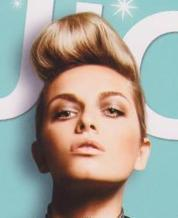
\includegraphics[scale=0.6]{Graphics/000005.jpg}
    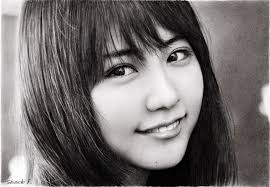
\includegraphics[scale=0.6]{Graphics/00000013_orig.jpeg}

    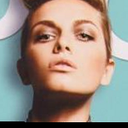
\includegraphics[scale=0.6]{Graphics/000004.png}
    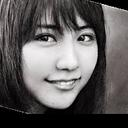
\includegraphics[scale=0.6]{Graphics/00000013.jpeg}
    \end{center}
    \caption{Preprocessing examples. Original images containing faces(top) and results after preprocessing steps(bottom)}\label{FIG:preprocess}
\end{figure}

In this section we deals with the preprocessing steps on face sketches and photos, which were applied separately before the training of model. By experiments of a few weeks, we found this part crucial to the performance of model. 
The first step of data refinement was to detect every faces for each image. By excluding images not containing recognized faces, we could get rid of 20\% of bad examples in sketch database. Then, we applied `facial landmark detection' for the detected faces, in order to get further information concerning the direction of head in the images. We utilized the `dlib' framework ~\cite{dlib} for those two steps.
Next, we rotated the images to have faces aligned vertically using the detected locations of two eyes.
Finally, the images were cropped to have faces in center and 30\% of the width of head margins on both sides. The cropped images have 128 by 128 size in the end of preprocessings. Those steps were applied to both sketch and photo images to make them consistent in any attributes other than it is sketch or photo. 

After some experiments we found that the model was learning to put smile on the generated photo from sketch images even when the original sketch images were not smiling. This seemed to be originated from the fact that images in photograph have smile in most case, while sketch images haven't. Since this was undisired effect, we reduced the ratio of smiling faces in the photograph dataset. This process was done by checking attributes file which Celebrity A dataset provided to see wether given image is smiling or not and using only one images per 20 smiling images.

\subsection{Generating Sketch Images}
% TODO: add content to or remove this part

\endinput
